\documentclass[a5paper, 10pt]{article}

% Текст
\usepackage[utf8]{inputenc} % UTF-8 кодировка
\usepackage[russian]{babel} % Русский язык
\usepackage{indentfirst} % красная строка в первом параграфе в главе
% Отображение страниц
\usepackage{geometry} % размеры листа и отступов
\usepackage{listings}
\usepackage{color}

\geometry{
	left=12mm,
	top=25mm,
	right=15mm,
	bottom=17mm,
	marginparsep=0mm,
	marginparwidth=0mm,
	headheight=10mm,
	headsep=7mm,
	nofoot}
\usepackage{afterpage,fancyhdr} % настройка колонтитулов
\pagestyle{fancy}
\fancypagestyle{style}{ % создание нового стиля style
	\fancyhf{} % очистка колонтитулов
	\fancyhead[LO, RE]{Лабораторная работа № 3 } % название документа наверху
	\fancyhead[RO, LE]{Жёсткая фильтрация} % название section наверху
	\fancyfoot[RO, LE]{\thepage} % номер страницы справа внизу на нечетных и слева внизу на четных
	\renewcommand{\headrulewidth}{0.25pt} % толщина линии сверху
	\renewcommand{\footrulewidth}{0pt} % толцина линии снизу
}
\fancypagestyle{plain}{ % создание нового стиля plain -- полностью пустого
	\fancyhf{}
	\renewcommand{\headrulewidth}{0pt}
}
\fancypagestyle{title}{ % создание нового стиля title -- для титульной страницы
	\fancyhf{}
	\fancyhead[C]{{\footnotesize
			Министерство образования и науки Российской Федерации\\
			Федеральное государственное автономное образовательное учреждение высшего образования
	}}
	\fancyfoot[C]{{\large 
			Санкт-Петербург, 2024
	}}
	\renewcommand{\headrulewidth}{0pt}
}

% Математика
\usepackage{amsmath, amsfonts, amssymb, amsthm} % Набор пакетов для математических текстов
%\usepackage{dmvnbase} % мехматовский пакет latex-сокращений
\usepackage{cancel} % зачеркивание для сокращений
% Рисунки и фигуры
\usepackage[pdftex]{graphicx} % вставка рисунков
\usepackage{wrapfig, subcaption} % вставка фигур, обтекая текст
\usepackage{caption} % для настройки подписей
\captionsetup{figurewithin=none,labelsep=period, font={small,it}} % настройка подписей к рисункам
% Рисование
\usepackage{tikz} % рисование
\usepackage{circuitikz}
\usepackage{pgfplots} % графики
% Таблицы
\usepackage{multirow} % объединение строк
\usepackage{multicol} % объединение столбцов
% Остальное
\usepackage[unicode, pdftex]{hyperref} % гиперссылки
\usepackage{enumitem} % нормальное оформление списков
\setlist{itemsep=0.15cm,topsep=0.15cm,parsep=1pt} % настройки списков
% Теоремы, леммы, определения...
\theoremstyle{definition}
\newtheorem{Def}{Определение}
\newtheorem*{Axiom}{Аксиома}
\theoremstyle{plain}
\newtheorem{Th}{Теорема}
\newtheorem{Lem}{Лемма}
\newtheorem{Cor}{Следствие}
\newtheorem{Ex}{Пример}
\theoremstyle{remark}
\newtheorem*{Note}{Замечание}
\newtheorem*{Solution}{Решение}
\newtheorem*{Proof}{Доказательство}
% Свои команды
\newcommand{\comb}[1]{\left[\hspace{-4pt}\begin{array}{l}#1\end{array}\right.\hspace{-5pt} } % совокупность уравнений
% Титульный лист
\usepackage{csvsimple-l3}
\newcommand*{\titlePage}{
	\thispagestyle{title}
	\begingroup
	\begin{center}
		%		{\footnotesize
			%			Министерство образования и науки Российской Федерации\\
			%			Федеральное государственное автономное образовательное учреждение высшего образования
			%		}
		%		
		\vspace*{6ex}
		
		{\small
			САНКТ-ПЕТЕРБУРГСКИЙ НАЦИОНАЛЬНЫЙ ИССЛЕДОВАТЕЛЬСКИЙ УНИВЕРСИТЕТ ИТМО	
		}
		
		\vspace*{2ex}
		
		{\normalsize
			Факультет систем управления и робототехники
		}
		
		\vspace*{15ex}
		
		{\Large \bfseries 
			Лабораторная работа № 3
		}
\vspace*{2ex}
	{\Large \bfseries 
			
"Жёсткая фильтрация"
		}
\vspace*{2ex}
		
		{\normalsize
			по дисциплине Частотные методы
		}

	\end{center}
	\vspace*{20ex}
	\begin{flushright}
		{\large 
			\underline{Выполнила}: студентка гр. \textbf{R3238}\\
			\begin{flushright}
				\textbf{Нечаева А. А.}\\
			\end{flushright}
		}
		
		\vspace*{5ex}
		
		{\large 
			\underline{Преподаватель}: \textit{Перегудин Алексей Алексеевич}
		}
	\end{flushright}	
	\newpage
	\setcounter{page}{1}
	\endgroup}

\begin{document}
	\titlePage
	\pagestyle{style}
\newpage

\section{Задание. Жёсткие фильтры.}
Зададимся числами $a = 1$, $t_1 = 0$, $t_2 = 2$ такими, что $t_1 < t_2$, и рассмотрим функцию $g$ такую, что $g(t) = a$ при $t \in [t_1, t_2]$ и $g(t) = 0$ при других $t$.\\
\\
 Выберем большой интервал $T = 20$ и маленький шаг дискретизации $dt$, соответствующий разбиению рассматриваемого интервала на 1000 точек. Зададим массив времени на отрезке $t = [-T/2,T/2]$ и найдем массив значений $g$ рассматриваемой функции на множестве точек $t$. Зададим зашумленную версию сигнала как
$$u = g + b \cdot (rand(size(t))-0.5) + c \cdot \sin (d \cdot t)$$

Выполним жёсткую фильтрацию указанного сигнала. Для выполнения фильтрации будем поступать так: будем находить Фурье-образ сигнала $u$, затем обнулять его значения на некоторых (выбранных нами) диапазонах частот, затем восстанавливать сигнал с помощью обратного преобразования.


\begin{figure}[h]
\center{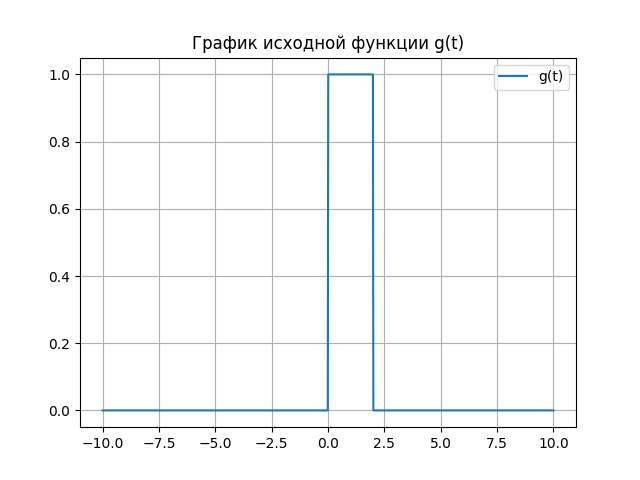
\includegraphics[width=0.85\linewidth]{pic/g_orig.png}}
\caption{График исходной функции $g(t)$.}
\end{figure}

\begin{figure}[h]
\center{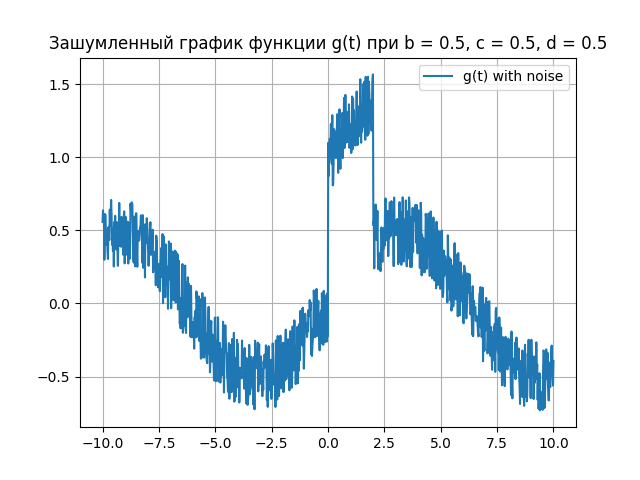
\includegraphics[width=0.85\linewidth]{pic/n_0.5_0.5_0.5.png}}
\caption{График функции $g(t)$ с шумами при $b = 0.5, c = 0.5, d = 0.5$.}
\end{figure}

\subsection{Убираем высокие частоты}

Пусть $c = 0$









\subsection{Убираем специфические частоты}










\subsection{Убираем низкие частоты?}





\newpage
\section{Задание. Фильтрация звука.}



%Для визуализации был написан код на языке \textit{Python}. \\
%Код расположен на \href{https://github.com/a-nechaeva/practical_Linal/tree/main/lab4}{\textbf{GitHub}}.


\end{document}













